% !TeX root = ../__ylc_main.tex

\chapter{相关研究综述}

本章从三个方面来介绍关于学生的认知建模以及大语言模型在此方面的应用的研究背景。第一部分介绍了学生认知建模的相关研究,包括知识追踪、认知诊断等方面。第二部分介绍了大语言模型的相关研究,包括大语言模型的基本原理、发展历程等。第三部分介绍了大语言模型在教育领域的应用,包括大语言模型在教育领域的应用前景、研究进展等。

\section{知识追踪和认知诊断}

随着信息技术的发展,人们逐渐开始探究如何用计算机来辅助教学,提高教学效率。在近几年大语言模型出现之前,人们就已经在使用传统的统计、机器学习,乃至近期的深度学习模型来试图刻画学生的知识掌握情况、对学生能力进行建模,并对学生未来的表现进行预测。知识追踪(Knowledge Tracing,KT)和认知诊断(Cognitive Diagnosis, CD)是这方面的两个重要研究方向。它们旨在通过对学生的学习过程和认知状态进行建模和分析,为教师提供个性化的教学支持和指导。

这两类工作都基于固定的题库和固定的知识点划分。知识追踪 的主要任务是根据学生的解题历史预测他们正确回答其他问题的可能性;认知诊断 的主要任务是根据学生的解题历史评估他们对各个知识点的掌握情况。

\subsection{知识追踪}

人类通过教学来传授知识的能力是人类智能的重要方面之一。人类教师可以通过观察学生的知识掌握情况,根据学生的需求定制教学。随着在线教育平台的兴起,机器也同样需要追踪学生的知识,为他们量身定制学习体验。这类研究问题被称为知识追踪(KT)问题。有效解决知识追踪问题将开发计算机辅助教育应用的潜力,为智能辅导系统、课程学习和学习材料推荐等智能教育系统提供算法解决方案。此外,从更广泛的角度来看, 知识追踪问题中所关注的“学生”可以是任何类型的智能体,包括人类和人工智能 Agent。因此,KT 的潜力可以推广到任何寻求为智能(如机器学习模型)定制学习体验的机器教学应用场景\cite{abdelrahman2023knowledge}。KT对在线学习系统和学生都具有重要意义。首先,KT模型能够开发个性化的自适应学习系统。一旦掌握了学生的知识状态,学习系统就可以为不同的学生定制更合适的学习方案,从而可以根据学生的熟练程度进行教学。其次,学生自己也可以更好地了解他们的学习过程,并逐渐更多地关注掌握不熟练的技能\cite{liu2019exploiting}。

知识追踪(Knowledge Tracing,KT)基于对学生行为序列的建模来获取学生的认知状态并预测学生未来的学习表现。知识追踪任务旨在根据学生的历史学习行为,实时地建模学生的知识状态,从而预测学生未来的学习成绩。

知识追踪已经研究了几十年,早期与KT相关的研究可以追溯到20世纪70年代末;但是\citet{corbett1994knowledge} 的工作是第一个引入“知识追踪”这一概念的研究,他们利用贝叶斯网络来模拟学生学习过程,这被称为贝叶斯知识追踪。随后越来越多的研究者开始关注与知识追踪相关的研究。例如,许多逻辑模型已被应用于KT,包括学习因子分析(Learning Factor Analysis)和表现因素分析(Performance Factor Analysis)。近年来,深度学习逐渐被应用与对KT任务的研究,因为它具有强大的提取和表示特征的能力,以及发现复杂结构的能力。例如,深度知识追踪引入了循环神经网络(RNN)进入KT任务,并被发现明显优于以前的方法。之后,通过考虑学习序列的各种特征,更多的方法将各种类型的神经网络引入到KT任务中。此外,由于实际应用的要求,KT模型的许多变体也不断开发,KT已经广泛应用于许多教育场景\cite{liu2021survey}。

\subsection{认知诊断}

在智能教育系统领域,认知诊断(Cognitive Diagnosis, CD)\cite{liu2023new}是一项基本而重要的任务,其目的是通过学生表现评估预测过程来衡量学生对特定知识概念的掌握程度。认知诊断有很多可能的应用,包括计算机自适应测试、定向培训和练习题目推荐系统。认知诊断系统一般都涉及一个题目-概念矩阵(也被称为 Q-矩阵),Q-矩阵经过专家的标注,用来表示每一道练习题中涉及到了哪些知识、概念或能力。多数认知诊断模型大多依赖于由领域专家标注的标记完全的 Q-矩阵来训练模型,这些研究侧重于增强响应记录的挖掘过程,以获得更好的诊断结果。

一个典型的认知诊断过程如图\ref{fig:cd_example}中例子所示。例如,在练习题目 v3 中考察了知识概念 k3 和 k5。根据 CD 模型的诊断,学生 u2 对这两个概念的熟练程度高于 u1,因为 u2 在练习题中回答正确,而 u1 回答错误。很明显,全标注 Q 矩阵在 CD 模型的可解释性(即诊断报告)方面起着至关重要的作用\cite{chen2024disentangling}。

\begin{figure}
    \centering
    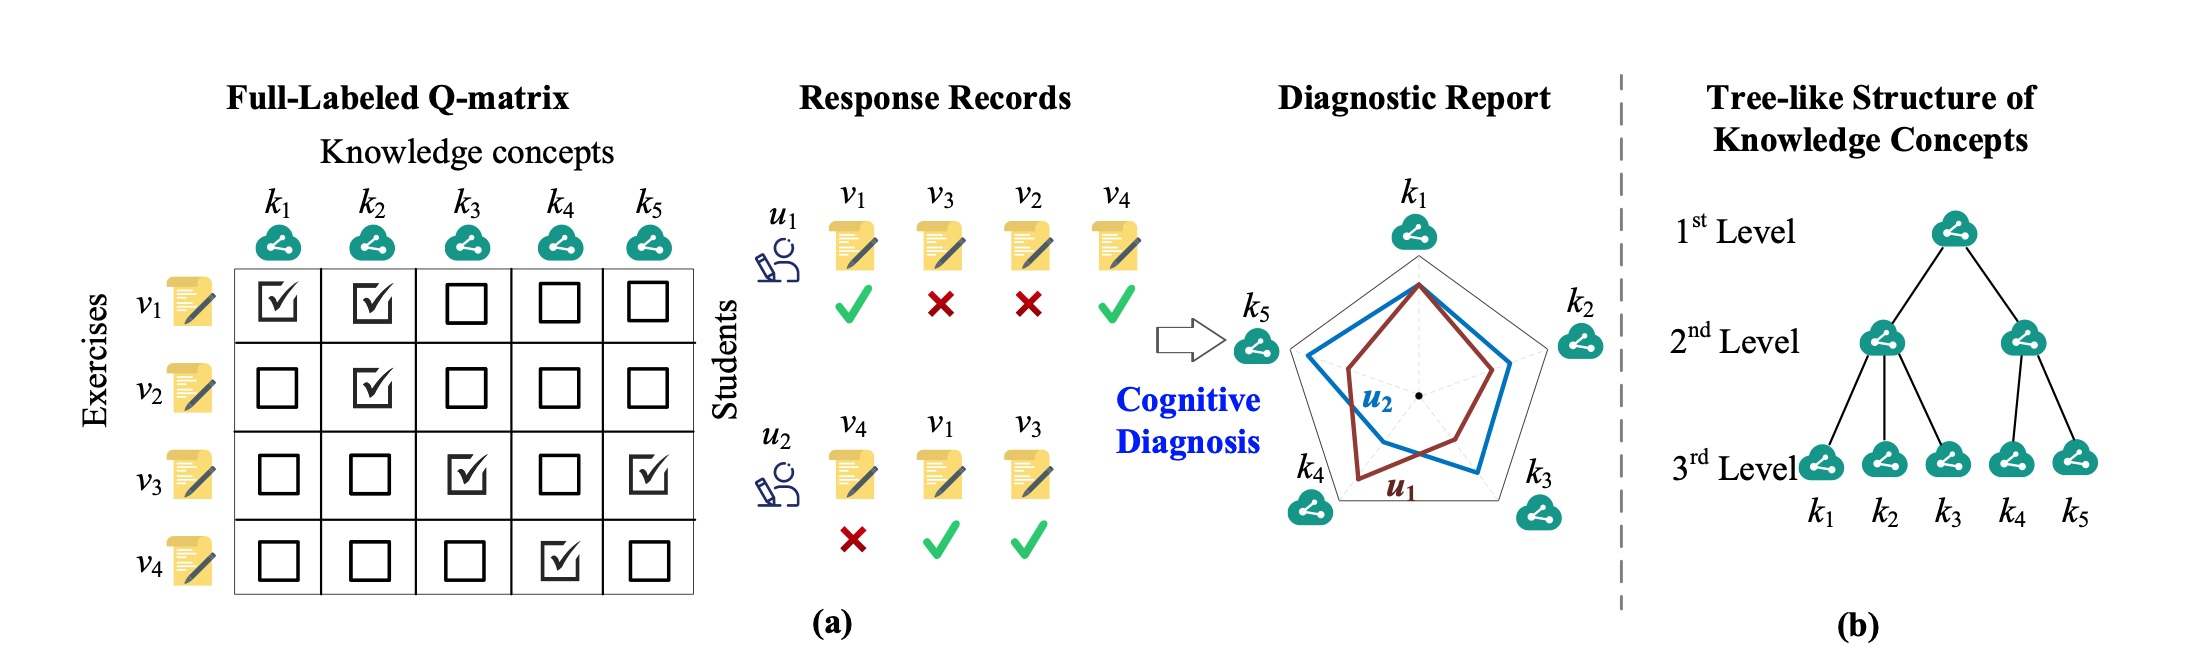
\includegraphics[width=\linewidth]{cd_example.png}
    \caption*{CD 任务流程示例,引自\citet{chen2024disentangling}。(a) 展示了使用专家注释的完全标注的 Q-矩阵来进行认知诊断的例子。(b) 为该过程依赖的概念的树状结构,与Q-矩阵比可以以较低成本完成标注。}
    \caption{认知诊断过程示例}
    \label{fig:cd_example}
\end{figure}

\subsection{知识追踪与认知诊断的局限性}

知识追踪与认知诊断都是利用计算机技术和算法来建模学生的认知状态和知识掌握情况进行建模的尝试。虽然已经取得了比较好的效果,但是二者仍然存在着不少局限性,很难广泛应用到教学场景中。

首先,两种方法中判断学生是否会做一道题,都是记录学生做题结果的“对与错”。这种方法并不能非常精确地判断学生是否真正理解了知识点、是否真正会做这道题,只能判断学生是否得到了正确答案,哪怕是学生刚好猜对的。这种方法只适用于选择题、判断题等解题过程比较简单、能够通过正误来准确定位到学生具体欠缺的能力或知识的题目类型,对于解答题就束手无策了,一些开放性题目如填空题和作文,也无法有效处理。其次,两种方法都是基于固定的题库和固定的知识点划分。这种方法无法适应学生的个性化需求,也无法适应教学内容的多样性。基于常见 KT 算法的个性化教学只能在题库里面选择合适的题目,而无法根据学生的实际需求生成新的题目或引入题库外的题目,实现真正的个性化教学;而由于 CD 算法的效果非常依赖对题目的标注,基于 CD 的个性化教学在引入新的题目的时候,需要人类教师标注对应的 Q-矩阵,成本较高。虽然目前有一些新的研究可以通过学习学生解题历史记录和少量(10\%-20\%)打了标签的题目,自动地对其他题目所考察的知识点和难度进行标注\cite{chen2024disentangling},但是这种方法仍然离不开人类专家的标注,且标注的成本仍然较高。

最重要的是,KT 和 CD 的方法也不能跟踪学生具体的解题过程和思路,无法进行更细粒度的分析。例如对于常见的数学解答题而言,解答的过程往往需要很多步推理、综合运用了一系列数学知识和能力。对于这类问题,学生的解题过程和思路往往比答案更重要,因为仅凭结果的正误无法推断出发生错误的步骤,更不能定位错误的根本原因到学生哪一知识的掌握比较薄弱。但 KT 和 CD 无法对这些信息进行有效的提取和分析。要想有效分析解答题的解题过程对学生能力的体现,就需要借助新的方法和工具了。


\section{认知过程的建模}

在 KT、CD 等通过学生历史做题的正误来建模学生的知识掌握情况的方法不同,认知过程的建模则是通过对学生的解题过程进行建模,用来解释大脑的认知结构以及解决问题的认知过程背后的内部知识表示机制。认知过程的建模是一种更加细粒度的建模方法,可以帮助我们更好地理解学生某次解题过程内部的认知过程,从而更好地进行个性化教学。比如\citet{wang2010cognitive} 的研究,提出了一套数学的认知模型,严谨地表示和刻画人类解决问题的过程。在他们看来,解决问题是大脑的一个认知过程,它为给定的问题寻找解决方案,或找到达到给定目标的路径。当一个问题的目标被确定后,解决问题可以被视为内存空间中的搜索过程,用于查找一组解决方案目标和一组替代路径之间的关系。研究者认为这一研究可以帮助未来一代认知计算方法的发展,以及为未来能够思考、学习和感知的新型认知计算机奠定基础。这篇研究中提出的思维过程的数学模型对于本研究所要实现的目标而言过于复杂繁琐,但其方法启发了本研究中解题过程刻画方法的设计。

\begin{figure}
    \centering
    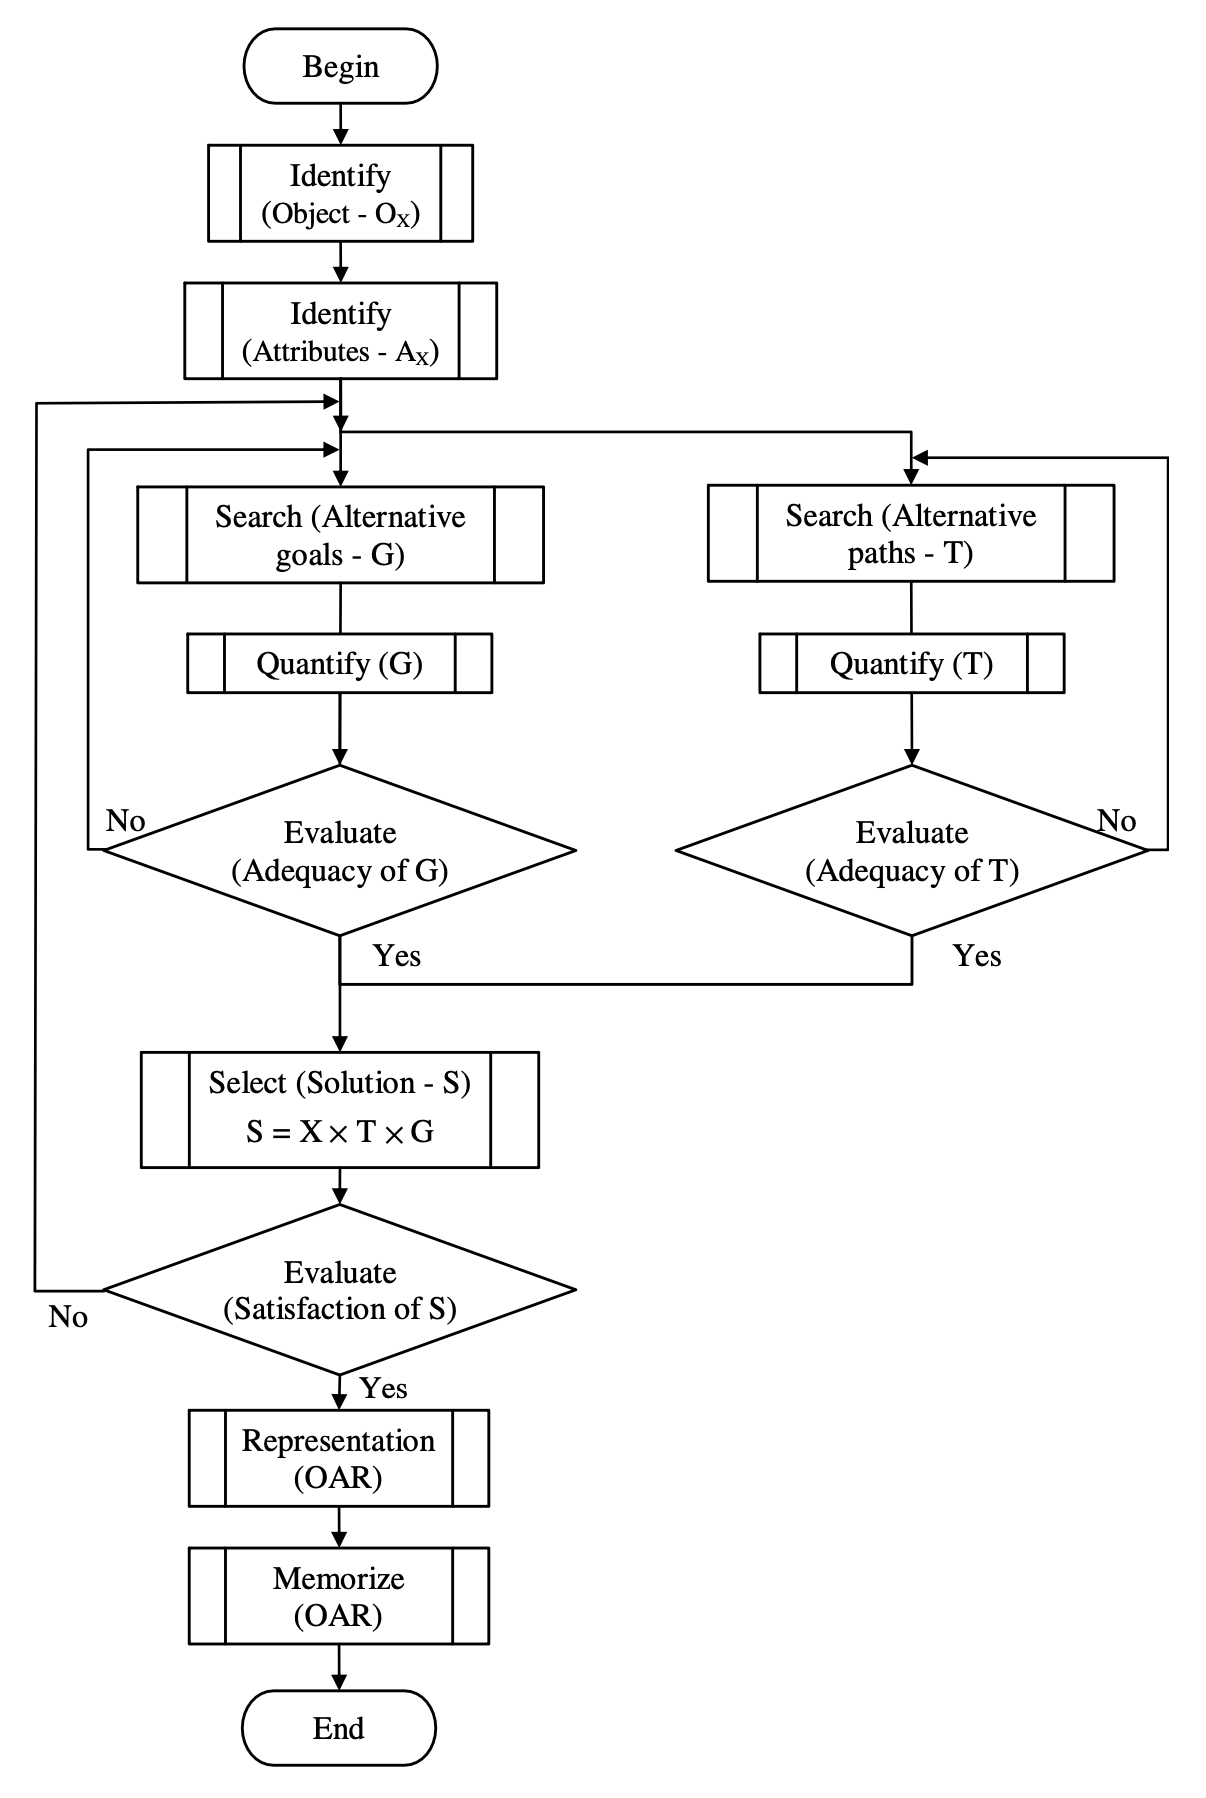
\includegraphics[width=0.5\linewidth]{cognitive_process.png}
    \caption*{一个普通的问题解决过程建模示例,引自\citet{wang2010cognitive}。其中解决问题的认知过程可以分为定义问题、搜索目标和解决路径、生成解答、选择合适的解答、表示问题解决结果这五个步骤。}
    \caption{问题解决过程建模示例}
    \label{fig:cognitive_process}
\end{figure}

\section{大语言模型}

语言模型通过对文本序列的概率进行建模,以预测给定输入后最有可能的输出序列。近年来,基于transformer架构\cite{vaswani2017attention}的语言模型在参数量和训练数据量方面不断增长,近年来不断出现更新、能力更强的大语言模型。例如LaMDA\cite{thoppilan2022lamda},PaLM\cite{anil2023palm},和 OpenAI 公司的 GPT-3 模型\cite{brown2020language}、在线大语言模型聊天服务 ChatGPT\cite{abdullah2022chatgpt},以及目前最新的支持文本和图片多模态输入的 GPT-4\cite{achiam2023gpt}。 这类被称作大语言模型 (LLM) 的大参数量模型 (千亿到万亿级别的参数量) 系统相继涌现。它们已经展示了在不需要重新训练的情况下,能够广泛适应新任务的强大泛化能力。

为了让LLM按需执行任务,用户需要精心编写自然语言指令,人们更常见地称这种输入给 LLM 的自然语言指令为提示词(prompts)。提示词可以提供少量示例(few-shot examples),也可以仅提供任务描述而不包含示例。随着人们在日常场景或工程开发上对 LLM 的使用逐渐增多,提示工程成为了与大型语言模型进行有效对话所需的一项日益重要的技能,人们也已经总结出了一系列经验上的提示词工程技术,可以提供可重复使用的解决方案\cite{white2023prompt}。LLM在多种新任务中的优异表现表明,它们在学习大规模语料的过程中,将语言中丰富的语义知识嵌入模型内部,而输入提示词的过程则可以被视作将这些知识提取出来。

LLM为人机交互带来了新的机遇\cite{bommasani2021opportunities}。它们能够处理终端用户多样化的自然语言表达,更准确地理解用户意图,使得即使缺乏专业知识的用户也能更容易地构建AI应用。此外,LLM内部蕴含的丰富知识还能作为多模态数据的粘合剂,利用其他模态的数据增强其情境理解能力,从而更好地执行任务。

总之,LLM的发展现状展示了它在自然语言处理和多模态数据集成方面的巨大潜力,通过较强的对语言的理解和生成能力,为人工智能的广泛应用提供了坚实的基础。本研究利用LLM语义理解能力和数学逻辑能力在智能教育领域的应用。通过给 LLM 提供学生的解题过程的详细内容、题目本身与标准解答图等数据,我们可以使它有效地理解学生的解题过程,将其翻译成我们规定好的结构化的数据结构,对学生认知进行建模,并以自然语言输出解题报告进行个性化的辅导。

\section{LLM 在教育领域的应用}

随着大语言模型的不断发展,在教育领域中,大型语言模型(LLM)的应用前景广阔且充满潜力\cite{gan2023large}。这些应用不仅能够提升教学质量,还能显著改善学生的学习体验。

首先,LLM能够根据学生的学习需求和兴趣,提供个性化的学习内容和推荐,从而帮助学生更有效地学习和成长。通过分析学生的学习数据和行为模式,LLM可以设计出独特的学习路径和资源,满足每个学生的个性化需求。对于特定的学科(比如英语),大模型也可以根据需求生成高质量的练习题,使得学生的练习不再受限于固定的题库。

此外,LLM作为教师的辅助工具,能够为教师提供智能教学支持平台。这些平台可以生成内容和建议,帮助教师设计教学活动、监控学生的学习进度,并提供个性化的教学支持。教师可以利用LLM生成的内容和建议,进行更有针对性的教学,从而提高教学效率和效果。

在教育评估方面,LLM也展现了巨大的潜力。通过自动分析学生的作业、考试等学习数据,LLM能够提供关于学生学习进展的评估和反馈。这不仅提高了评估的效率,还能为教师和学生提供及时的反馈,帮助他们及时调整教学和学习策略,从而促进学生的学习和成长。

然而,LLM在教育中的应用也面临一些挑战。首先是数据隐私和安全问题。智能教育需要收集和分析大量学生数据,这引发了对学生隐私和数据安全的担忧。因此,建立健全的数据管理和保护机制,确保学生数据的安全和合法使用,是智能教育发展的关键。其次是技术基础设施和资源的需求。智能教育的实施需要充足的技术基础设施和资源支持,包括网络连接、计算设备、教育软件等。然而,目前一些地区和学校可能面临技术条件和资源匮乏的问题,这限制了智能教育的广泛应用和推广。制定相关的法律法规,确保智能教育在带来教育效益的同时,遵循伦理原则和社会公平,是下一步推广智能教育时的重要社会议题。